% tex file for convolution
\par  \indent Our study has a event related neurological stimulus, not block stimulus which was discussed in class. We predict the hemoglobin response (HR) related to this type of neurological stimulus, since the methods in class were much better for block stimulus. Moreover our stimulus (as is the case in event-related stimulus studies) wasn't evenly split. We developed a few other functions to take this into account, and will probably implement one more procedure before the end.

\par  The three approaches we will have explored (the first two already completed) address modeling the HR from the neural stimulus. \textbf{(1)} We first implemented the standard block-stimulus paradigm related \texttt{np.convolve} function (which failed to take into account the non-trivial times of stimulus). Np.convolve utilities FFT (Fast Fourier Transforms). \textbf{(2)} Next, we developed a function that doesn't utilize FFT, but allows for dis-continuous events of stimulus (discontinuous, being non-uniform stimulus timing). We used a continuous HR function to model the response (whereas \texttt{np.convolve} uses a discrete HR function).\textbf{(3)} Our next project (\textit{which really should be included in the "Future plans" section}) is to utilize the strength of FFT by splitting up the time into 60 milliseconds intervals (a very small time metric), and then uses \texttt{np.convolve} and some rounding of the stimulus response occurrences to get another candidate for the Hemoglobin response related to the neurological stimulus. This procedure would use the strength of FFT, and wouldn't be hurt by assumptions of time since the HR model isn't super precise and there is a good amount of variance.
    
\par   For \textbf{(2)} and \textbf{(3)} we have to scale back down to the image capturing time frame (2 seconds) [Figure: \ref{fig:convolution}].


\begin{figure}[ht]
\centering
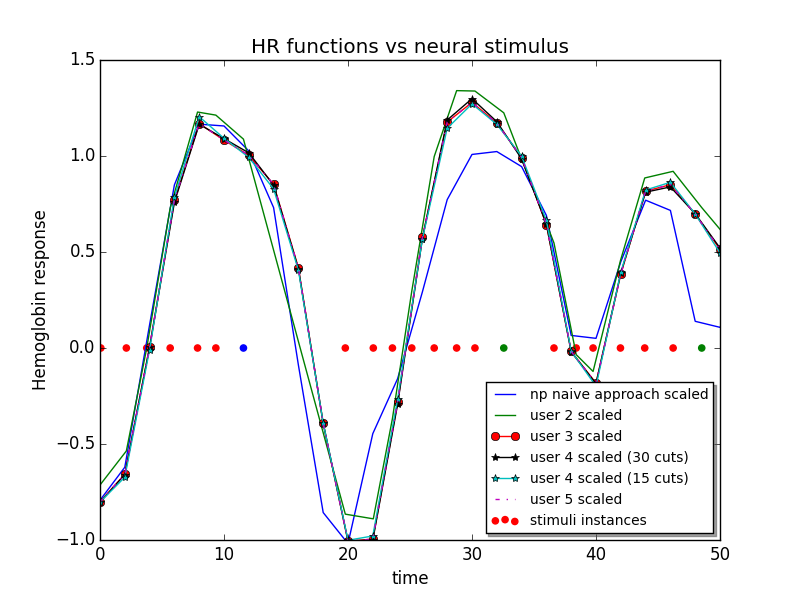
\includegraphics[scale=0.5]{images/convolution_vs_neural_stimulus} 
\caption{Different convolution function vs the Nueral stimulus}
\label{fig:convolution}
\end{figure}

